\documentclass[english,usenames,dvipsnames]{beamer}
\usetheme{Boadilla}
\usepackage[utf8]{inputenc}
\usepackage{caption}
\usepackage{appendixnumberbeamer}
\usepackage{verbatim}
\definecolor{myred1}{RGB}{255,50,0}
\definecolor{myblue1}{RGB}{0,100,255}
\definecolor{mygreen1}{RGB}{34,139,35}


\title{The Effect of Non-Competes on Productivity Growth through Spinouts and R\&D}
\author{Nicolas Fernandez-Arias}
\date[Dec 14 2017]{Student Macro Workshop, Dec 14, 2017}

\begin{document}
	
\frame{\titlepage}

\begin{frame}{Introduction}
\label{Introduction}
\begin{itemize}
	\item A \textbf{non-compete agreement} is a clause in an employment contract preventing the employee from working for a competitor (including founding a competing firm) during specified time span after leaving current employer
	\begin{itemize}
		\item Often limited in geographic scope
		\item Sometimes have attached a \emph{buyout clause} that allows the employee to free himself, though rare except managers (Rauch 2015)
	\end{itemize}
	\item A \textbf{spinout} of a firm is a new firm founded by an employee of the initial firm
	\begin{itemize}
		\item E.g. Fairchild semiconductor spinouts form basis of SV \hyperlink{fairchild_spinouts}{\beamerbutton{detail}}
		\item Note: NOT a \emph{spinoff}, which is a subsidiary of a company which is sold off
	\end{itemize}
	\item \textbf{Question this project seeks to answer}: What is the effect of non-competes on productivity growth and welfare?
\end{itemize}
\end{frame}

\begin{frame}{Motivation}
\label{Motivation1}
\begin{itemize}
	\item Empirical importance of non-competes (survey data)
	\begin{itemize}
		\item 20\% of US labor force currently under a non-compete, higher for knowledge workers (Starr 2017) \hyperlink{incidence_ind_oc}{\beamerbutton{by industry and occupation}} 
		\item 88\% of companies with less than \$50 million in sales require non-competes (Leonard 2001)
		\item VC firms require non-competes for 90\% of founders of companies they finance (Kaplan \& Stromberg 2000)
	\end{itemize}
	\item Empirical importance of entry and employee spinouts in particular:
	\begin{itemize}
		\item 25\% of aggregate productivity growth due to entrants (Akcigit \& Kerr 2017)
		\item In Brazil, employee spinouts account for between 15-30\% of entrants; larger, grow faster than other entrants (Muendler et al. 2012)
	\end{itemize}
\end{itemize}
\end{frame}

\begin{frame}{Motivation: current policy issue}
\label{Motivation2}
\begin{itemize}
	\item Differing enforcement across states \hyperlink{differing_enforcement}{\beamerbutton{map}} 
	
	\item Literature has tentatively endorsed the view that Silicon Valley, CA displaced Rt. 128, MA as high-tech hub due to non-enforcement (starting with Saxenian 1994, Gilson 1999, etc.)
	\item Policymakers converging to belief that not enforcing is key to creating high-tech hub 
	\begin{itemize}
		\item 2015 - Hawaii passes law precluding enforcement of non-competes for "technology workers"
		\item Several states considering weakening enforcement explicitly in an effort to imitate California (e.g. Massachusetts)
	\end{itemize}
\end{itemize}
\end{frame}

%%%%%%%%%%%%%%%%%%%%%%%%%%%%%%%%
% NEED TO FIX THIS SLIDE!!! %%%%
%%%%%%%%%%%%%%%%%%%%%%%%%%%%%%%%%
\begin{frame}{Theory: big picture}
\label{theory_big_picture}
\begin{itemize}
	\item Schumpeter 1942, Arrow 1962, etc.: if knowledge is not excludable, it will be underproduced in competitive equilibrium because no private benefit to agent incurring costs of production
	\item Intellectual property laws (e.g. patents) makes knowledge excludable
	\item Patent literature: optimal level of excludability? Dynamic efficiency vs. static monopoly distortion tradeoff (Nordhaus 1967, etc.)
	\item Similar economics here
	\item Why use non-competes instead of patents or non-disclosure agreements (NDAs) to protect intellectual property?
	\begin{itemize}
		\item Some knowledge is difficult to patent (e.g., early stage knowledge, c.f. discussion in Hellmann-Perotti 2005)
		\item NDAs are hard to enforce
		\item Sometimes NDAs are de facto non-competes under "inevitable disclosure" doctrine (in enforcing states)
		\item Suggestive survey evidence that non-competes are used to protect trade secrets \hyperlink{incidence_bi}{\beamerbutton{detail}} 
	\end{itemize}
\end{itemize}
\end{frame}

%%%%%%%%%%%%%%%%%%%%%%%%%%%%%%%%%%%%%%%%%%%%%%%
% Add some more citations here if have time %%%%%
%%%%%%%%%%%%%%%%%%%%%%%%%%%%%%%%%%%%%%%%%%%%%
\begin{frame}{Existing theoretical work}
\begin{itemize}
\item Advantages of non-competes:
\begin{itemize}
	\item more employer investment in R\&D (e.g., Shankar-Ghosh 2013)
	\item more employer investment in employee human capital (e.g., Shi 2017)
	\item reduce socially inefficient creative destruction (Shi 2017)
\end{itemize}
\item Disadvantages of non-competes:
\begin{itemize}
	\item less employee reallocation to better match (e.g. Shankar-Ghosh 2013, Shi 2017)
	\item less employee investment in own human capital (Garmaise 2011) 
	\item static monopoly distortion of production (Rauch 2015)
\end{itemize}
\item Note: in theory optimal contract would mitigate these disadvantages are avoided through buyouts / renegotiation, but empirically not used for average tech worker / researcher (Rauch 2015)
\end{itemize}
\end{frame}

\begin{frame}{Existing empirical work}
\label{empirical_work1}
\begin{itemize}
	\item Survey: Bishara-Starr 2016 "The Incomplete Noncompete Picture"
	\item In non-enforcing regimes:
	\begin{itemize}
		\item Employment / payroll / business formation grows more in response to exogenous increases in the supply of VC funding (Samila-Sorenson 2011)
		\item More workforce mobility (Fallick et al. 2006, Garmaise 2011, Marx et. al 2009)
		\item Less market concentration (Kang-Fleming 2017)
		\item Employees have higher wages (Chang et al. 2017)
	\end{itemize}
\end{itemize}
\end{frame}

\begin{frame}{Existing empirical work (cont.)}
\begin{itemize}	
	\item In addition to shortcomings cited in Bishara-Starr 2016...
	\item ...empirical work based on comparing outcomes depending on enforcement regime (even that based on exogenous variation) cannot identify aggregate effect if there are \textbf{cross-regime spillovers}
	\item Direct evidence of brain drain from Michigan to non-enforcing regions after accidental policy change in late 1985 (Marx 2015) 	
	\begin{itemize}
		\item After Michigan began enforcing, hazard rate of migration from patent holders to non-enforcing regimes \emph{doubled}
		\item More pronounced for those with more patents \& more valuable patents
	\end{itemize}
\end{itemize}
\end{frame}


\begin{comment}
\begin{frame}{Proposal}
\begin{itemize}
	\item Write fully dynamic structural model quantifying some of the tradeoffs identified in the theoretical literature (and some new) 
	\item Calibrate model of R\&D and  \textbf{taking spillovers seriously}
	\begin{itemize}
		\item If control for spillovers, can discipline innovation, spinout parameters using relative outcomes by enforcement regime
		\item To control for spillovers, need (at least) model mapping spillovers to relative outcomes
		\item Do not observe all relevant spillovers, so need a model predicting unobserved spillovers based on observed (e.g. derive entrepreneur spillovers from worker spillovers by calibrating a model of relocation decision to observed worker spillovers)
		\item Once spillovers properly accounted for, leftover relative outcomes across enforcement regimes discipline innovation, spinout parameters
	\end{itemize}
	\item Policy counterfactuals (can do with one region)
\end{itemize}
\end{frame}
\end{comment}

%% NEED TO MAKE SURE THIS IS NESTED IN TRADEOFF SLIDE!%%%%
%%%%%%%%%%%%%%%%%%%%%%%%%%%%%%%%%%%%%%%%%%%%%%%%%%%%%%
\begin{frame}{This paper}
\begin{itemize}
	\item Model quantifies a specific tradeoff (closest to Shankar-Ghosh 2013)
	\item Advantages of non-competes
	\begin{itemize}
		\item more employee investment in knowledge capital 
		\item prevent employees from spinning out and engaging in socially inefficient creative destruction
		\item prevent entrants from engaging in socially inefficient arms race (entrants are small, incumbent is large)
	\end{itemize}
	\item Disadvantages of non-competes
	\begin{itemize}
		\item prevent more productive employee spinouts from forming
		\item monopoly distortion on R\&D 
	\end{itemize}
\end{itemize}
\end{frame}

\section{Data}
\begin{frame}{Data}
\label{Data}
\begin{itemize}
	\item Have:
	\begin{itemize}
		\item Crunchbase full dataset: free dataset, 100,000+ startups (mostly founded in the last 20 years \hyperlink{crunchbase_founding_dates_coverage}{\beamerbutton{chart}}), information on founders and funding rounds. Some missing data, but more coverage of early stage startups than competing (expensive) datasets
		\item Moments from empirical work: e.g. brain drain in Marx 2015
		\item Survey data from Starr 2017 on prevalence of non-competes
		\item Data on strength of non-compete enforcement from Bishara 2011
	\end{itemize}
	\item Need / want: 
	\begin{itemize}
		\item Previous employment / occupation of founders in Crunchbase dataset. VentureOne has this, but it is not free.
		\item Better industry / product information classification -- need to merge with Crunchbase by firm name
		\item LEHD data would be great for comparing outcomes across different enforcement regions...but hard to come by. 
	\end{itemize}
\end{itemize}
\end{frame}

\section{Model}
\subsection{Overview}

\begin{frame}{Model overview}
\begin{itemize}
	\item Quality ladders model (ultimately based on Grossman-Helpman 1991)
	\item Endogenous productivity growth through improved quality of intermediate goods
	\item Quality improvements result from labor allocated to R\&D 
	\item R\&D workers at incumbent form spinouts to compete in R\&D race
	\item Creative destruction
\end{itemize}
\end{frame}

%%%%%%%%%%%%%%%%%%%%%%%%%%%%%%%%%%%%%%%%%%
%%% GOING TO NEED TO FIX ALL OF THIS SHIT TOMORROW MORNING!!!%%% 
%%%% BUT I THINK YOU WILL GET SOME USEFUL FEEDBACK! THIS HOPEFULLY WILL NOT BE A DISASTER!!!%%%%


\begin{frame}{Model: Intermediate goods production}
\begin{itemize}
	\item Continuum of intermediate goods, indexed by $j\in J = [0,1]$
	\item Denote frontier quality of good $j$ by $q_j$, amount produced by $c_j$
	\item Each good produced with technology
	\begin{align*}
	c_j = \overline{q} l_j
	\end{align*}
	where $\overline{q} = \int_0^1 q_j dj$ is the average quality level of the economy
	\item At a given point in time, each good has a monopoly producer
	\item Across goods, monopolistic competition
\end{itemize}
\end{frame}

\begin{frame}{Model: Final good production}
\begin{itemize}
	\item Final good is produced using labor and a continuum of intermediate goods $j\in[0,1]$ with production technology
	\begin{align*}
	C(t) &= L(t)^{\beta}\Bigg(\Big(\int_0^1 q_j(t)^\beta 
	c_j^{1-\beta}(t)dj \Big)^{1/(1-\beta)}\Bigg)^{1-\beta} \\
		&=  L(t)^{\beta}\int_0^1 q_j(t)^\beta c_j^{1-\beta}(t)dj
	\end{align*}
	where $q_j$ is quality, $c_j$ is quantity
	\item Restricts labor share to be related to markup $\mu = 1/(1-\beta)$
	\item Can relax this using Grossman et. al 2016
	\item CRS implies zero profits so no need to consider ownership
\end{itemize}
\end{frame}

\begin{frame}{Model: R\&D race timing}
\begin{table}
	\begin{tabular}{p{0.8\textwidth}}
		\centering
		Participant in the R\&D race for good $j$ begins with monopoly on good $j$ R\&D \\
		$\downarrow$\\
		Hires R\&D labor; at rate $\nu$ per unit of R\&D labor hired, an employee acquires ability to open rival R\&D lab (but not to compete directly on product market). \\
		$\downarrow$\\
		This worker becomes part of mass $n_j$ and leaves the lab (replaced by someone who values the chance of learning the R\&D process)\\ 
		$\downarrow$\\
		At rate $\tau$, agents' non-competes expire, adding to the mass $m_j$ \\
		$\downarrow$\\
		At some point, either incumbent or entrant wins patent race, restarting the process 
	\end{tabular}
\end{table}
\end{frame}

\begin{frame}{Model: R\&D race (cont.)}
\begin{itemize}
	\item Laws of motion for $m_j,n_j$
	\begin{align*}
	\dot{n}_j &= \nu l_j^{RD} - \tau n_j \\
	\dot{m}_j &= \tau n_j
	\end{align*}
	\item Note that $(q_j,m_j,n_j)$ is the state of product $j$	
\end{itemize}
\end{frame}

\begin{frame}{Model: R\&D technology}
\begin{itemize}
	\small
	\item $z_I$,$z_E$ units of labor yields innovations at Poisson rate (for incumbents and entrants, respectively)
	\begin{align*}
	R_I(z_I;\overline{z}) &= \chi_I z_I \phi(\overline{z}) \\
	R_E(z_E;\overline{z}) &= \chi_E z_E \phi(\overline{z}) 
	\end{align*}
	where 
	\begin{align*}
	\overline{z}^j = \int_0^{m_j} z^j(\ell)d\ell + z^j_I
	\end{align*}
	is total innovation effort on $j$, with (endogenous) mass $m$ of entrants indexed by $\ell$.
	\item Total arrival rate of innovations at $j$ is $\zeta_j = (\chi_I z^j_I + \chi_E \int_0^{m_j} z^j(\ell)d\ell) \phi(\overline{z}^j)$
	\item Entrant productivity of R\&D $\chi_E$ weakly greater than incumbent productivity $\chi_I$
	\item $\phi(z)$ decreasing, $z\phi(z)$ increasing
	\item Entrant $\ell$ can hire $z\le\xi$ units of R\&D labor (in equilibrium $z(\ell) = \xi$)
\end{itemize}
\end{frame}



\begin{frame}{Model: Workers}
\begin{itemize}
	\item Unit mass continuum of risk-neutral individuals indexed by $i\in I =[0,1]$, with objective
	\begin{align*}
	U = \int_0^{\infty}\exp(-\rho t)c(t)dt
	\end{align*}
	where $c(t)$ is final goods consumption at $t$.
	\item Individuals can supply labor to final goods production ($l^F$), intermediate good production ($l^I$) and R\&D ($l^{RD}$) such that 
	\begin{align*}
	l_t^F+ l_t^I + l_t^{RD} = 1
	\end{align*}
	\item Aggregate labor market satisfies (where $L_t^k = \int_I l_t^k(i)di$)
	\begin{align*}
	L_t^F + L_t^I + L_t^{RD} = 1
	\end{align*}
\end{itemize}
\end{frame}

\begin{frame}{Worker optimization timeline}
\begin{table}
	\begin{tabular}{p{0.8\textwidth}}
		\centering
		Allocates labor to R\&D and final and intermediate good production (indifferent) \\
		$\downarrow$\\
		While performing R\&D for good $j$ hit by knowledge shock with intensity $\nu$ per unit of R\&D labor supplied to $j$ \\
		$\downarrow$\\
		No longer works for good $j$ until next step on ladder (because already has knowledge) \\
		$\downarrow$\\
		At rate $\tau$, hit by non-compete expiry shock \\
		$\downarrow$\\
		Provided $m_j < M_t(q,n)$ (``free entry" mass of entrants), enters R\&D race 
	\end{tabular}
\end{table}
\end{frame}

\begin{frame}{Worker optimization}
\small
\begin{itemize}
	\item Workers indifferent between occupations (Final goods, intermediate goods, R\&D)
	\item From assumptions on intermediate and final goods production, get closed form for final goods wage  $\overline{w}_t = \Gamma(\beta) \overline{q}_t$
	\item Indifference condition implies intermediate goods wage $w^I_t = \overline{w}_t$ 
	\item R\&D wage at product $j$ depends on state of the product, which is $(q,m,n)$
	\item Indifference condition
	\begin{align*}
	w_t(q,m,n) + \nu W^{NC}_t(q,m,n) &= \overline{w}_t
	\end{align*}
	where $W^{NC}_t(q,m,n)$ is the value of the knowledge (bound by a non-compete)
	\item Since $w_t(q,m,n) < \overline{w}_t$, in equilibrium workers immediately leave employer once knowledge is attained 
	\item Note: this indifference condition implies that value functions $A,W^F,W^{NC}$ do not scale with $q$
\end{itemize}
\end{frame}


\begin{frame}{Intermediate goods firms optimization}
\begin{itemize}
	\small
	\item Let $\tilde{q}$ denote $qe^{-gt}$ where $g$ is growth rate on BGP 
	\item Value function of \textbf{incumbent} is $A_t(q,m,n) = e^{gt}A(\tilde{q},m,n)$
	\item Flow profits: $\pi(\tilde{q}) = \tilde{\pi}\tilde{q}$ in eq.
	\item HJB equation:
	\footnotesize
	\begin{align*}
	(\rho - g)A(\tilde{q},m,n) &= \pi(\tilde{q}) - g\tilde{q}A_{\tilde{q}}(\tilde{q},m,n)- \tau n A_n(\tilde{q},m,n) + \tau n A_m (\tilde{q},m,n) \\
							   & + \max_{\textcolor{myred1}{z}} \Big\{\chi_I\textcolor{myred1}{z}\phi(\textcolor{myred1}{z}+ \textcolor{mygreen1}{\overline{z}_E(\tilde{q},m,n)})\overbrace{\textcolor{myblue1}{\Big(A((1+\lambda)\tilde{q},0,0)-A(\tilde{q},m,n)\Big)}}^{\text{NPV of successful innovation}} \\
							   & - w(\tilde{q},m,n)\textcolor{myred1}{z} +\nu(\textcolor{myred1}{z}+\textcolor{mygreen1}{\overline{z}_E(\tilde{q},m,n)})A_n(\tilde{q},m,n) \\
							   &  - \chi_E\textcolor{mygreen1}{\overline{z}_E(\tilde{q},m,n)}\phi(\textcolor{myred1}{z}+\textcolor{mygreen1}{\overline{z}_E(\tilde{q},m,n)})A(\tilde{q},m,n)\Big \} 
	\end{align*}
	\normalsize
	\item $A_m,A_n<0$ and $A_{\tilde{q}} > 0$ in equilibrium
\end{itemize}
\end{frame}

\begin{frame}{Intermediate goods firms optimization (cont.)}
\begin{itemize}
	\small
	\item Value function of \textbf{entrant no longer bound by non-compete} is $W^{F}(\tilde{q},m,n)$
	\item HJB equation:
	\small
	\begin{align*}
	(\rho + \zeta(\tilde{q},m,n) - g)W^F(\tilde{q},m,n) &= - g\tilde{q}W^F_{\tilde{q}}(\tilde{q},m,n) \\ &+ (\nu \textcolor{mygreen1}{\overline{z}(\tilde{q},m,n)} - \tau n)W_n^F(\tilde{q},m,n) \\
	 & + \tau n W_m ^F (\tilde{q},m,n) \\ + \max_{\textcolor{myred1}{z}} \Big\{\chi_E\textcolor{myred1}{z}\textcolor{mygreen1}{\phi(\overline{z}(\tilde{q},m,n))} & \overbrace{\textcolor{myblue1}{\Big(A((1+\lambda)\tilde{q},0,0)-W^F(\tilde{q},m,n)\Big)}}^{\text{NPV of successful innovation}} \\
	& - w(\tilde{q},m,n)\textcolor{myred1}{z} \Big\} \\
	\end{align*}
	where $\zeta(\tilde{q},m,n)$ is the total arrival rate of innovations 
	\small
	\item $W^F_m,W^F_n<0$ and $W^F_{\tilde{q}} > 0$ 
	\item Entrants continue to enter until mass $M(\tilde{q},n)$, where $M(\tilde{q},n) = M_t(q,n)$
	\item Hence total entrant R\&D will be $\overline{z}_E(\tilde{q},m,n) = \xi \min (M(\tilde{q},n),m)$
\end{itemize}
\end{frame}

\begin{frame}{Intermediate goods firms optimization (cont.)}
\begin{itemize}
	\item Value function of \textbf{entrant bound by non-compete} is $W^{NC}(\tilde{q},m,n)$
	\item HJB equation:
	\small
	\begin{align*}
	(\rho + \zeta(\tilde{q},m,n) + \tau - g)W^{NC}(\tilde{q},m,n) &= - g\tilde{q}W^{NC}_{\tilde{q}}(\tilde{q},m,n) \\
	& + (\nu \overline{z}(\tilde{q},m,n)-\tau n)W_n^{NC}	\\
	& + \tau n W_m^{NC} + \tau W^F(\tilde{q},m,n) \\ 
	\end{align*}
	\small
	\item $W^F_m,W^F_n<0$ and $W^F_{\tilde{q}} > 0$ 
	\item Entrants continue to enter until a mass $m = M(\tilde{q},n)$, where $M(\tilde{q},n) = M_t(q,n)$
	\item Hence aggregate entrant R\&D will be $\overline{z}_E(\tilde{q},m,n) = \xi \min (M(\tilde{q},n),m)$
\end{itemize}
\end{frame}




\subsection{Equilibrium}
\begin{frame}{Recursive BGP Equilibrium}
\begin{itemize}
	\footnotesize
	\item Growth rate $g$, value functions $A(\tilde{q},m,n),W^F(\tilde{q},m,n),$ and $ W^{NC}(\tilde{q},m,n)$, ergodic distribution $dP(\tilde{q},m,n)$, R\&D wages $w(\tilde{q},m,n)$, production wage $\overline{w}$, prices and quantities of intermediate goods, free entry mass $M(\tilde{q},n)$, individual R\&D policies $z_I(\tilde{q},m,n)$ and $z_E(\tilde{q},m,n)$, total entrant R\&D $\overline{z}_E(\tilde{q},m,n) = \xi \min(M(\tilde{q},n),m)$, total R\&D $\overline{z}(\tilde{q},m,n) = z_I(\tilde{q},m,n) + \overline{z}_E(\tilde{q},m,n)$, production labor allocations $L^F$ and $L^I(j)$ such that:
	\begin{itemize}
		\footnotesize
		\item Value functions $A,W^F,W^{NC}$ solve HJB eqs, individual policy functions optimal given value functions
		\item Ergodic distribution $dP(\tilde{q},m,n)$ satisfies KF equation 
		\item Final and intermediate goods wage satisfy $\overline{w} = \Gamma(\beta)$
		\item R\&D wages satisfy indifference condition $w(\tilde{q},m,n) + \nu W^{NC}(\tilde{q},m,n) = \overline{w}$
		\item $M(\tilde{q},n)$ is smallest $m$ satisfying free entry condition $w(\tilde{q},m,n) = A(\tilde{q},0,0) - W^F(\tilde{q},m,n)$
		\item Labor resource constraint: $L^F + L^I + L^{RD} = 1$
		\item Growth $g$ is consistent with research policy functions: $g = \lambda \int \tilde{q} \zeta(\tilde{q},m,n)dP(\tilde{q},m,n)$
	\end{itemize} 
\end{itemize}
\end{frame}

\begin{frame}{Efficiency}
\begin{itemize}
	\item Worker indifference condition implies firm compensated (in expectation) for profits of future spinouts
	\item Franco-Filson 2006 logic suggests this may imply Pareto efficiency without non-competes
	\item However, equilibrium may still be inefficient as spinouts reduce monopoly power, shifting equilibrium along dynamic efficiency / static monopoly distortion tradeoff
	\item This introduces role for non-competes 
	\item Could introduce further role by making R\&D labor supply less elastic (infinitely elastic here due to indifference condition)
\end{itemize}
\end{frame}

\section{Extensions}
\begin{frame}{Next steps}
\begin{itemize}
	\item Solve model numerically -- challenging due to 3 state variables (expect equilibrium to exist, but have not proven)
	\item Add enforcing and non-enforcing regions, which requires answering...
	\begin{itemize}
		\item How does migration map into differential outcomes?
		\item How does observed migration map into relevant unobserved migration?
	\end{itemize}
	\item Calibration
	\begin{itemize}
		\item How to map migration in the data to migration in the model? Data not a BGP
	\end{itemize}
	\item Welfare analysis and optimal non-compete length
\end{itemize}
\end{frame}

% Appendix for figures

\appendix

\captionsetup[figure]{labelformat=empty}

\begin{frame}{Incidence of Non-competes}
\label{incidence_ind_oc}
\hyperlink{Motivation1}{\beamerbutton{back}}
\begin{figure}
	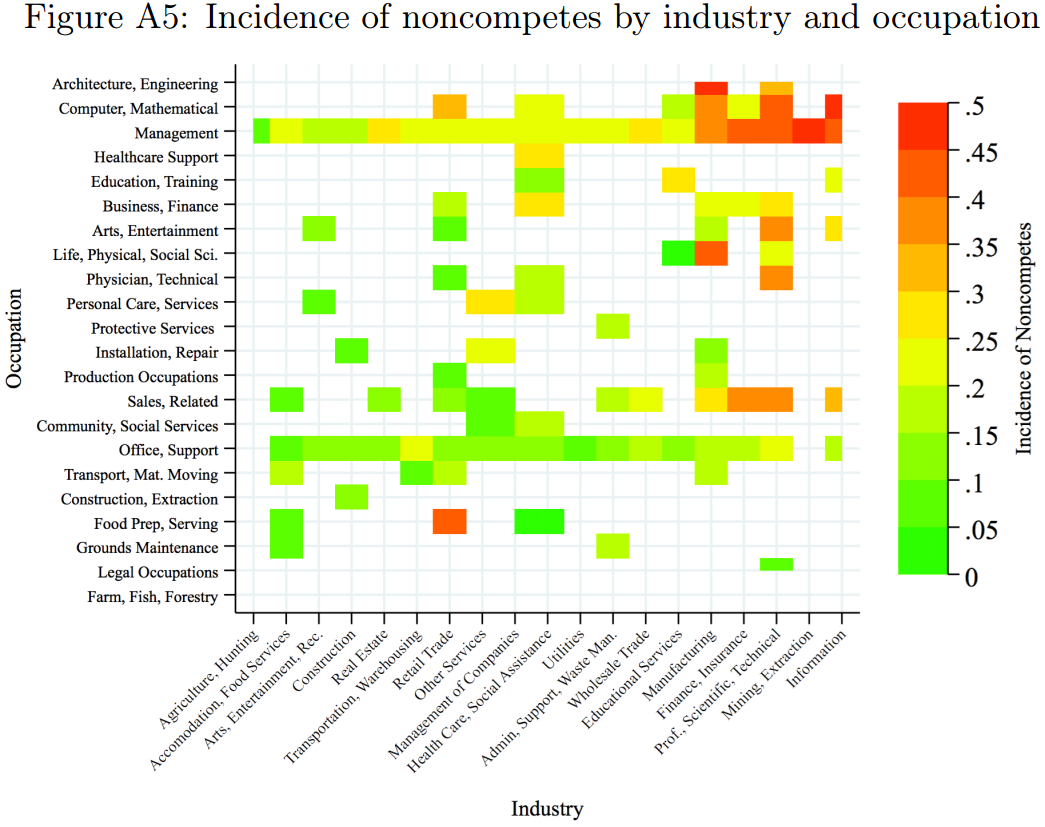
\includegraphics[scale=0.38]{figures/nc_incidence_industry_and_occupation}
	\caption{Source: Starr et al. 2017 (survey data)}
\end{figure}
\end{frame}

\begin{frame}{Incidence of Non-competes}
\label{incidence_bi}
\hyperlink{theory_big_picture}{\beamerbutton{back}}
\begin{figure}
	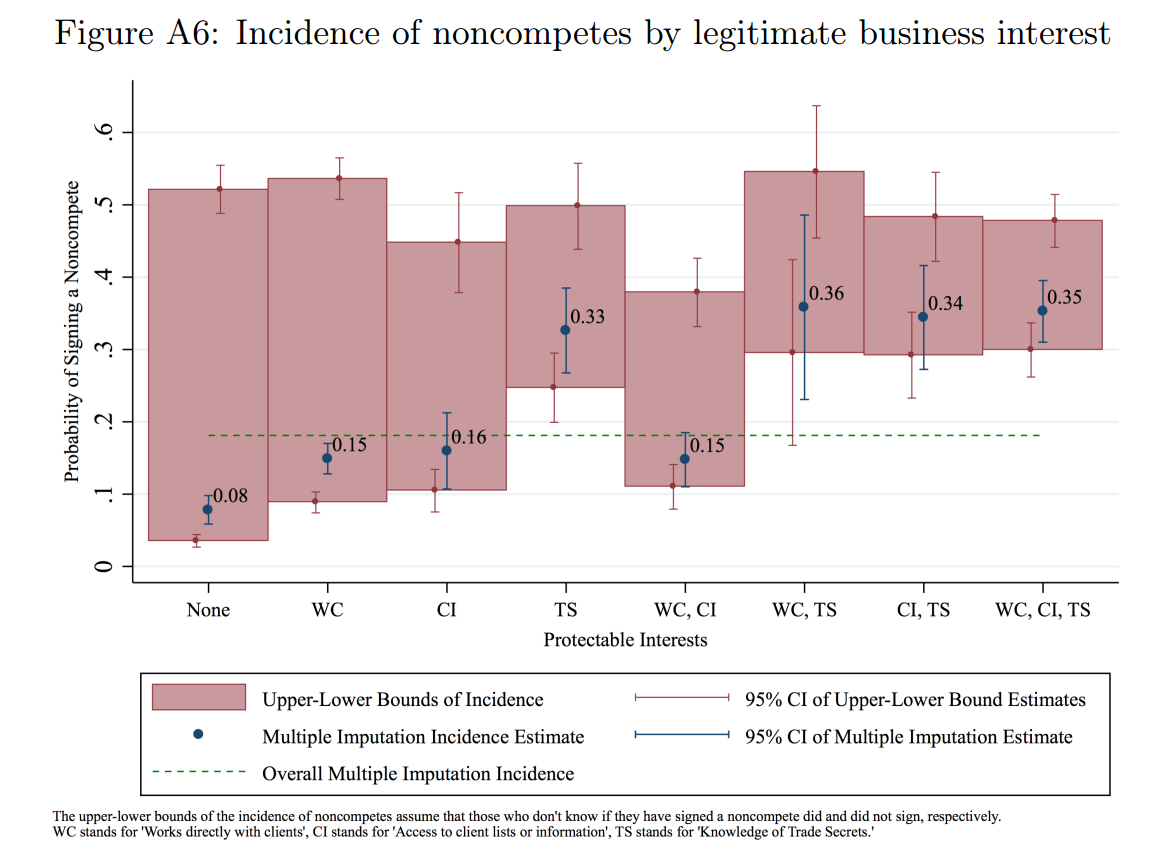
\includegraphics[scale=0.37]{figures/nc_incidence_business_interest}
	\caption{Source: Starr et al. 2017 (survey data)}
\end{figure}
\end{frame}

\begin{frame}{Incidence of Non-competes}
\label{incidence_enforceability}
\hyperlink{empirical_work1}{\beamerbutton{back}}
\begin{figure}
	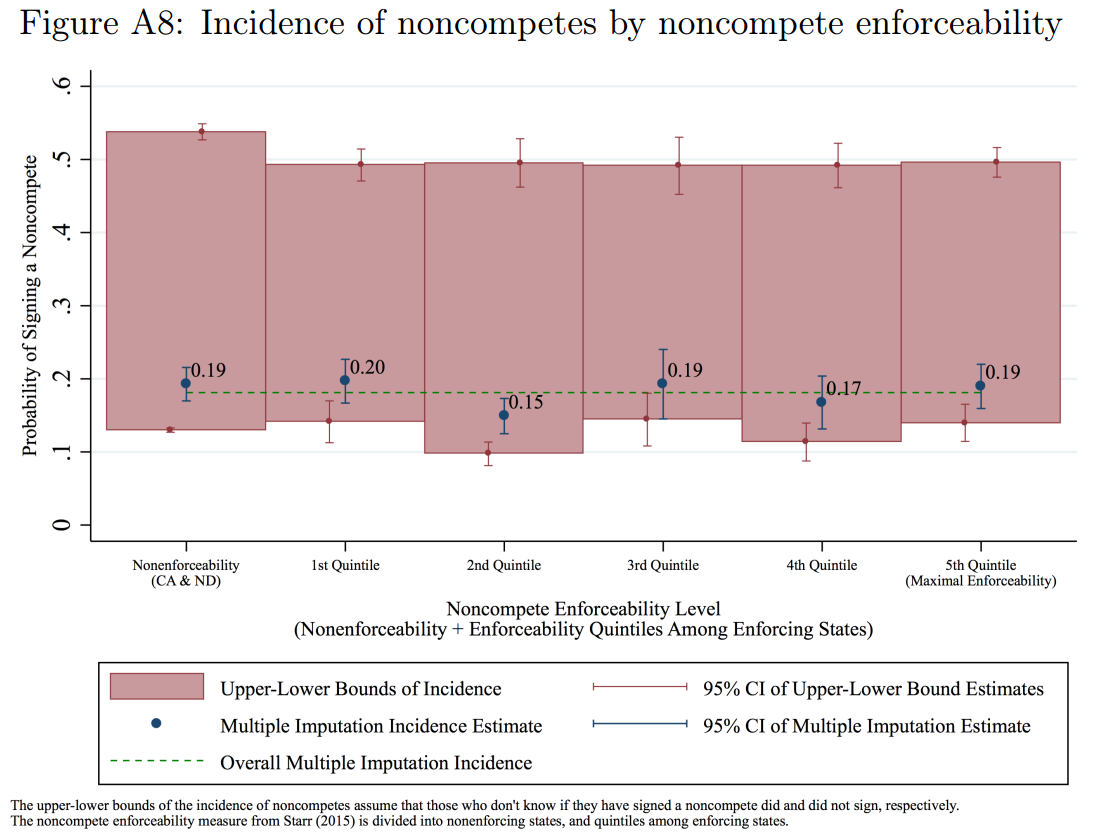
\includegraphics[scale=0.37]{figures/nc_incidence_enforceability}
	\caption{Source: Starr et al. 2017 (survey data)}
\end{figure}
\end{frame}

\begin{frame}{Spinouts of Fairchild Semiconductor}
\label{fairchild_spinouts}
\hyperlink{Introduction}{\beamerbutton{back}}
\begin{figure}
	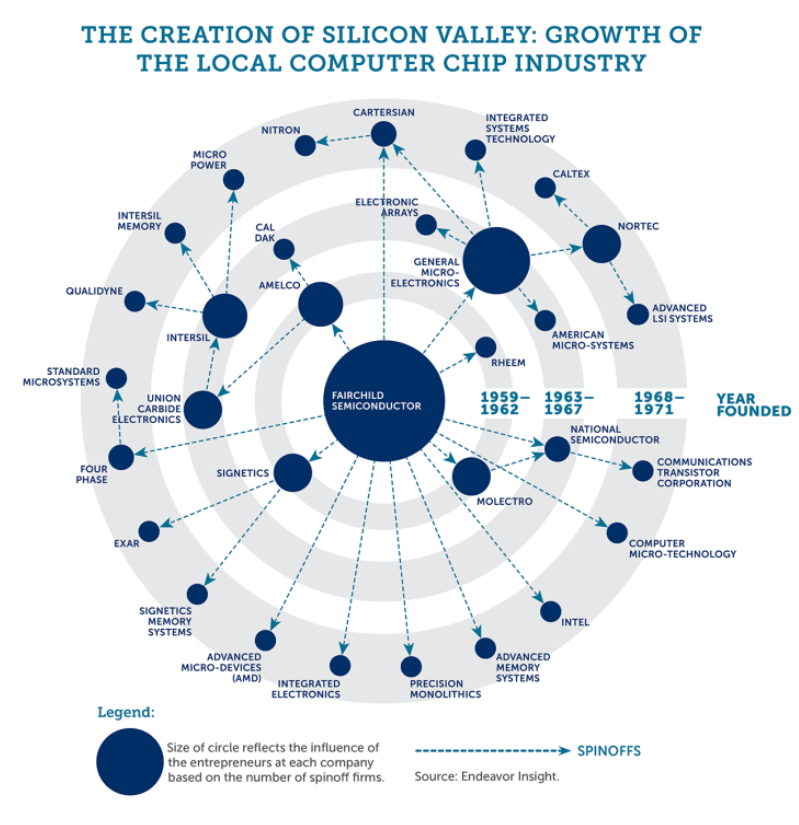
\includegraphics[scale=0.38]{figures/fairchild_spinouts}
	\caption{Source: Endeavor Insights}
\end{figure}
\end{frame}

\begin{frame}{Motivation: differing enforcement}
\label{differing_enforcement}
\hyperlink{Motivation2}{\beamerbutton{back}}
\begin{figure}
	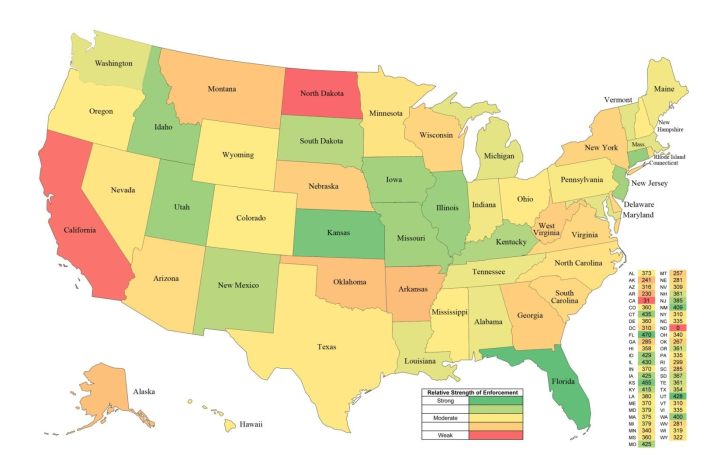
\includegraphics[scale=0.7]{figures/map_bishara_2009}
	\caption{Source: Bishara 2011}
\end{figure}
\end{frame}

\begin{frame}{Crunchbase data coverage}
\label{crunchbase_founding_dates_coverage}
\hyperlink{Data}{\beamerbutton{back}}
\begin{figure}
	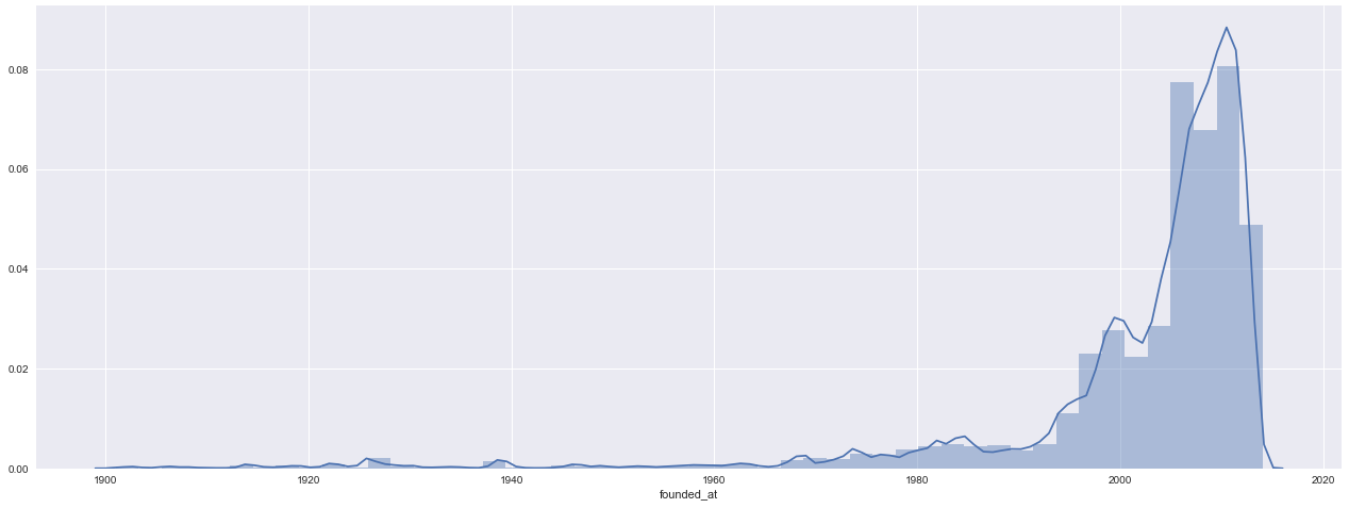
\includegraphics[scale=0.4]{figures/crunchbase_founding_dates}
	\caption{Figure: Histogram of founding dates for firms in Crunchbase dataset}
\end{figure}
\end{frame}









\end{document}